\documentclass[letterpaper, 11pt]{article}
\usepackage[letterpaper, margin=1.4in]{geometry}
\usepackage{amsmath, amssymb}
\usepackage{graphicx}
\usepackage{verbatimbox}
\usepackage{listings}
\lstset{
 basicstyle=\ttfamily,
 columns=fullflexible,
 frame=single,
 breaklines=true,
}
\usepackage{caption}
\usepackage{subcaption}

\title{Pacman API Specification}
\author{Team Houston\\ Jonathan Wang, Manu Maheshwari, Yanjun Yang,\\ Tianqi Ma, Youyi Wei, Jiang Lin}
\date{}

\setlength\parindent{0pt}

\begin{document}
\maketitle
We use the command and strategy design patterns for this game. The character objects (such as Pacman and ghosts) act according to strategies, and use commands to act in the game. All game objects also use the observable-observer design pattern to receive updates about the game state and handle interactions. Singleton design pattern were used when appropriate.

\section{Use Cases}
There are three groups of use cases for the Pacman game. We will look at the use cases and discuss how they will be handled by the API spec.
\begin{itemize}
    \item Pacman - how Pacman interacts with the game
  \begin{itemize}
    \item move in all directions based on user input - Pacman moves by a update strategy. The direction can be changed by the /switchDirection request
    \item does not go through walls - Pacman has an interact strategy that will handle collisions
    \item teleport through exits - Pacman has an interact strategy that will handle collisions
    \item eat food - Pacman has an interact strategy that will handle collisions
    \item eat afraid ghost - Ghost has an interact strategy that make it can be eaten by the Pacman
  \end{itemize}
  \item Ghosts - how ghosts interact with the game
  \begin{itemize}
    \item start in the jail - ghosts are initialized in the jail
    \item move based on strategy - ghosts each have an update strategy
    \item does not go through walls - ghosts have an interact strategy that will handle collisions
    \item teleport through exits - ghosts have an interact strategy that will handle collisions
    \item eat Pacman - ghosts have an interact strategy that will handle collisions
    \item eaten by Pacman when afraid - DispatchAdapter has an afraidTimer field that tracks when ghosts can be eaten by Pacman. The actual ghost-Pacman interaction is handled by the interact strategy
    \item go to jail - ghosts each have a jailTimer that tracks how long they stay in jail for 
  \end{itemize}
  \item Game - overall game behavior
  \begin{itemize}
    %\item display game objects - all game objects are observers stored in DispatchAdapter that will be passed to the view
    \item periodically spawn fruit - DispatchAdapter has a fruitTimer field that will determine when to add a fruit object to the observers
    \item track game values - DispatchAdapter has score and lives fields which will be updated during the game
  \end{itemize}

\end{itemize}

\section{View}
We have a single canvas in index.html where the game and game values will be displayed. In view.js there are functions to start and run the game and display game objects. The view makes requests to the controller to reset the game as well as update the game state. 

\begin{itemize}
  \item /resetGame - called on page load to setup the game
  \item /updateGame - called every 0.1 sec to receive game state. Game objects are drawn onto the canvas based on received data
  \item /switchDirection - called based on user input to change Pacman direction
\end{itemize}

Based on the returned data, the view draws the game objects onto the canvas. The ghosts and fruit are image files, and the remaining game objects are drawn using canvas functions. Display-only features that do not affect the game operation, such as flashing ghosts, blinking dots, and the Pacman animation are handled exclusively in the view.

\section{Controller}
The PacWorldController processes GET and POST requests and returns the JSON representation of the DispatchAdapter, which contains all the game objects in the PacWorld. The controller creates the DispatchAdapter and defines the REST endpoints \\ 

These are the supported requests handled by PacWorldController:
\begin{itemize}
  \item /resetGame - gets the canvas dimension and passes it to the DispatchAdapter; resets game values and resets all game objects to the starting positions
  \item /udpateGame - updates the game state with collisions, new locations, removed objects, etc.
  \item /switchDirection - takes user input to change the Pacman movement direction
\end{itemize}

The controller also gets and sets the port assigned by Heroku for hosting.

\section{Model}
The model includes the DispatchAdapter, commands, strategies, and game objects.

\subsection{DispatchAdapter}
The DispatchAdapter communicates with the model and the view. It contains the observers and values for the game. These values include:
\begin{itemize}
  \item Point dims - dimensions of game map
  \item static int gridSize - size of grid spaces for game scaling (static for easy access in concrete classes)
  \item int score - current game score
  \item int lives - current Pacman lives
  %\item int fruitTimer - cool down timer for fruit spawning
  \item int afraidTimer - time that Pacman can eat ghosts 
  \item int dotsLeft - record the number of remaining dots
  \item boolean gameOver - check whether the game is over
\end{itemize}

Methods in the DispatchAdapter include getters and setters for the fields as well as methods to run the game.
\begin{itemize}
  \item DispatchAdapter() - constructor
  \item setCanvasDims(Point dims) - set the canvas dimensions
  \item getCanvasDims() - get the canvas dimensions
  \item getGridSize() - get the game grid size
  \item getScore() - get the game score
  \item setScore(int score) - set the game score
  \item getLives() - get the remaining lives of the Pacman
  \item setLives(int lives) - set the remaining lives of the Pacman
  \item getAfraidTimer() - get the afraid time for the ghost
  \item setAfraidTimer(int afraidTimer) - set the afraid time for the ghost
  \item initializeGame() - reset observers and game values and add game objects as observers according to map layout
  \item initializeMap() - return 2D array representing layout of game objects
  \item updatePacWorld() - update game state, handling object movement and collisions
  \item sendCollisionCmd(AGameObject context) - send the collision command
  \item sendSwitchCmd(String switchInfo) - send the switch command
  \item switchDirection(String body) - read user input from body and change Pacman direction
  \item getDotsLeft() - get the number of dots left
  \item setDotsLeft(int dotsLeft) - set the number of dots left
 \end{itemize}
 
\subsection{Command}
The cmd package has an interface IGameObjectCmd. Three concrete commands CollisionCmd, SwitchCmd and UpdateCmd implement this interface. The hierarchy of this package is shown in figure \ref{figcmd}. 

\begin{figure}[htbp] 
  \centering
  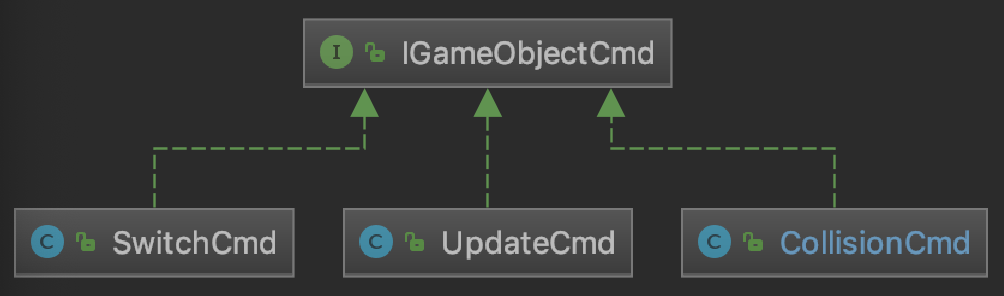
\includegraphics[width=.85\linewidth]{cmd.png} 
  \caption{Commands}
  \label{figcmd} 
\end{figure}

\begin{itemize}
  \item IGameObjectCmd - interface for all commands to allow game objects to act on game. The concrete commands will be UpdateCmd (object update), CollisionCmd (object collision), and SwitchCmd (Pacman direction). These three tasks can be performed with just the execute() method defined in the interface. 
  \begin{itemize}
    \item execute(AGameObject context) - allows context to act on the game state. The context object is the receiver that executes the command.
  \end{itemize}
  \item CollisionCmd - a concrete command executes the strategy when two objects meet.
  \begin{itemize}
  \item CollisionCmd(AGameObject object) - constructor
  \item execute(AGameObject context) - executes command on the dest object
  \end{itemize}
  \item SwitchCmd- a concrete command switches the strategy of the Pacman or a ghost
  \begin{itemize}
  \item SwitchCmd(String switchInfo, DispatchAdapter dis) - constructor
  \item execute(AGameObject context) - switches the strategy of the object
  \end{itemize}
  \item UpdateCmd- a concrete command updates the state of the Pacman or a ghost
  \begin{itemize}
  \item UpdateCmd(DispatchAdapter dispatchAdapter) - constructor
  \item execute(AGameObject context) - updates the states of the object
  \end{itemize}
\end{itemize}

\subsection{Strategy}
The strategy package has two interfaces - IUpdateStrategy and IInteractStrategy. Six concrete strategies for single object (GhostAfraidStrategy, GhostChaseStrategy, GhostRandomStrategy, GhostTrailStrategy, GhostTrapStrategy and PacmanUpdateStrategy) implement IUpdatesStrategy interface. Two concrete strategies for two-object interactions (GhostInteraction and PacmanInteraction) implement IInteractStrategy interface. The hierarchy of this package is shown in figure \ref{figstrategy}.

\begin{figure}[htbp] 
  \centering
  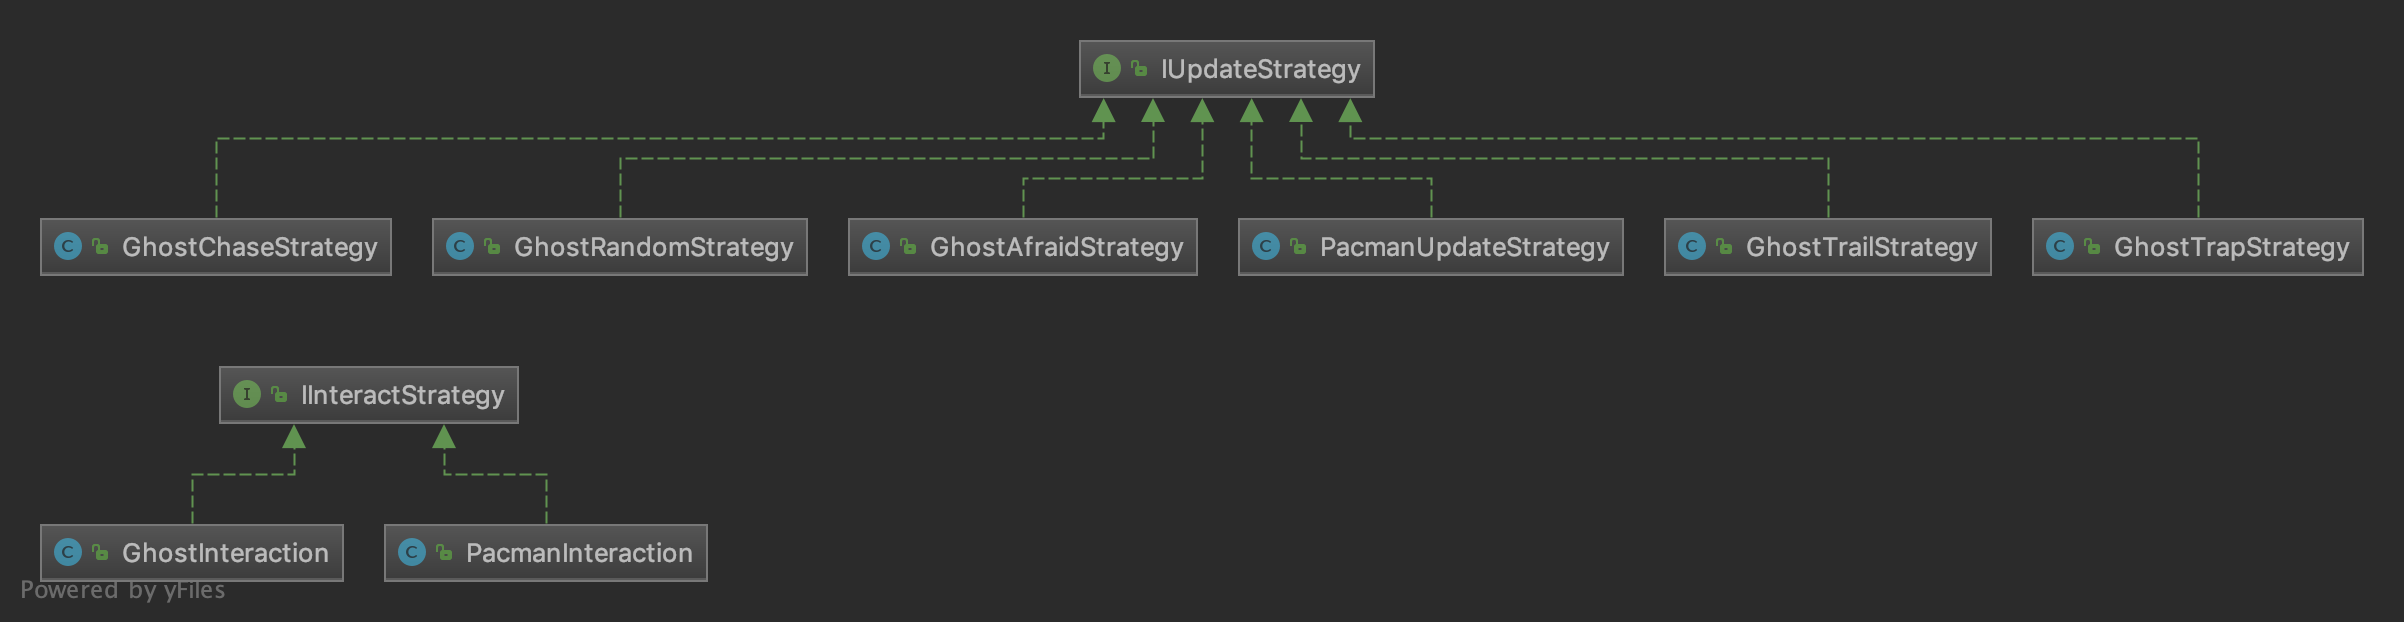
\includegraphics[width=0.98\linewidth]{strategy.png} 
  \caption{Strategies}
  \label{figstrategy} 
\end{figure}


\begin{itemize}
  \item IUpdateStrategy - interface for strategies that update individual game objects. Pacman will have a single update strategy that lets it move based on the user-specified direction. Ghosts will each have an update strategy for attacking and all use the same strategy when fleeing. No other game object has an update strategy, besides a null strategy.
  \begin{itemize}
    \item getName() - return update strategy name
    \item update(AGameObject context) - updates the state of the context object
  \end{itemize}  
  \item IInteractStrategy - interface for strategies that handle interaction between objects. All interactions in the game occur between two objects of different types. All interactions between two objects will be handled by one object. For instance, everything that occurs between Pacman and ghosts is handled by ghosts, and Pacman does not handle that interaction at all. This simplifies the number of cases to track and reduces the need for switching interaction strategies.
  \begin{itemize}
    \item getName() - return interact strategy name
    \item interact(AGameObject src, AGameObject dest) - handles interaction between src and dest objects
  \end{itemize}
  \item GhostAfraidStrategy - a concrete strategy to turn ghosts into the afraid state, during which the ghost can be eaten by the Pacman and the ghost will escape away from the Pacman.
  \begin{itemize}
  \item GhostAfraidStrategy() - constructor
  \item makeStrategy() - return a singleton of this strategy
  \item getName() - return the strategy name
  \item update(AGameObject gameObj) - updates the state of the context object
  \end{itemize}
  \item GhostChaseStrategy - a concrete strategy to make ghosts to chase and eat the Pacman.
  \begin{itemize}
  \item GhostChaseStrategy()- constructor
  \item makeStrategy() - return a singleton of this strategy
  \item getName() - return the strategy name
  \item update(AGameObject gameObj) - updates the state of the context object
  \end{itemize}
  \item GhostRandomStrategy - a concrete strategy to make ghosts walk in random directions.
  \begin{itemize}
  \item GhostRandomStrategy()- constructor
  \item makeStrategy() - return a singleton of this strategy
  \item getName() - return the strategy name
  \item update(AGameObject gameObj) - updates the state of the context object
  \end{itemize}
   \item GhostTrailStrategy - a concrete strategy to make ghosts trail.
  \begin{itemize}
  \item GhostTrailStrategy()- constructor
  \item makeStrategy() - return a singleton of this strategy
  \item getName() - return the strategy name
  \item update(AGameObject gameObj) - updates the state of the context object
  \end{itemize}
  \item GhostTrapStrategy - a concrete strategy to make ghosts trap the Pacman.
  \begin{itemize}
  \item GhostTrapStrategy()- constructor
  \item makeStrategy() - return a singleton of this strategy
  \item getName() - return the strategy name
  \item update(AGameObject gameObj) - updates the state of the context object
  \end{itemize}
 \item PacmanUpdateStrategy - a concrete strategy updates the state of the Pacman.
  \begin{itemize}
  \item PacmanUpdateStrategy()- constructor
  \item makeStrategy() - return a singleton of this strategy
  \item getName() - return the strategy name
  \item update(AGameObject gameObj) - updates the state of the context object
  \end{itemize}
\item GhostInteraction - a concrete strategy handle the interaction between the ghost and the Pacman.
  \begin{itemize}
  \item GhostInteraction(DispatchAdapter dis) - constructor
  \item makeStrategy() - return a singleton of this strategy
  \item getName() - return the strategy name
  \item interact(AGameObject src, AGameObject dest) - handle the interaction when two objects meet. The src object will impose the interaction strategy on the dest object and the dest object behavior will be affected by the src object interaction strategy
  \end{itemize}
  \item PacmanInteraction- a concrete strategy handle the interaction between the Pacman and other AGameObjects (wall, exit and food).
  \begin{itemize}
  \item PacmanInteraction(DispatchAdapter dis) - constructor
  \item makeStrategy() - return a singleton of this strategy
  \item getName() - return the strategy name
  \item interact(AGameObject src, AGameObject dest) - handle the interaction when two objects meet. The src object will impose the interaction strategy on the dest object and the dest object behavior will be affected by the src object interaction strategy
  \end{itemize}
\end{itemize}

\subsection{Game Objects}
The gameobject package has an abstract class AGameObject. Two abstract classes, ACharater and AFood, extend AGameObject. The abstract classes and the concrete classes are shown in figure \ref{fig1}. 

\begin{figure}[htbp] 
  \centering
  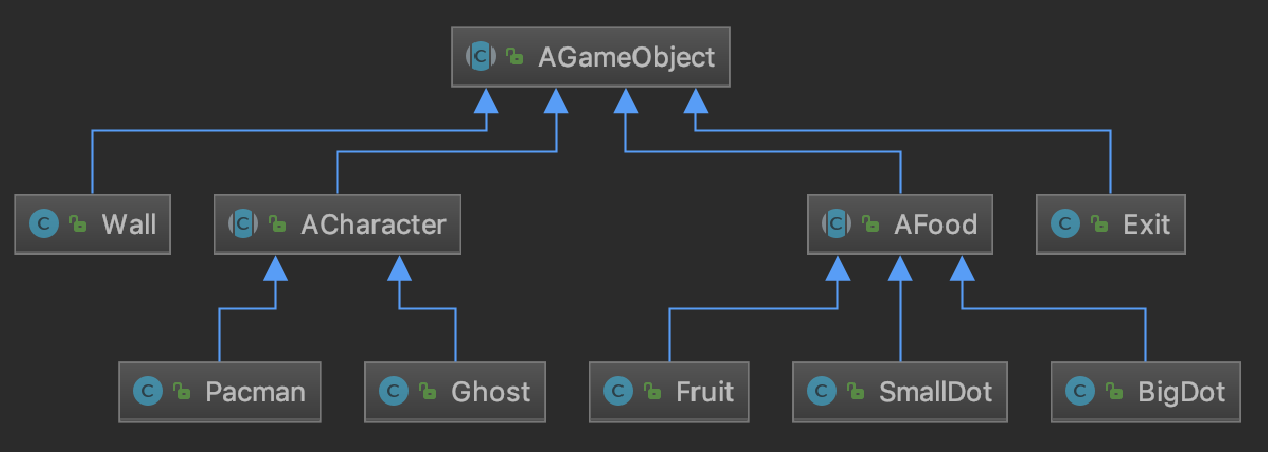
\includegraphics[width=.85\linewidth]{objects.png} 
  \caption{Game Objects}
  \label{fig1} 
\end{figure}

Several of the abstract and concrete classes do not have additional fields or methods from their parent class, but having the added class hierarchy simplifies object creation, and allows for extensible behavior. Each concrete class constructor sets the object size based on the DispatchAdapter gridSize. This allows for easy scalability with just one variable change. 

\begin{itemize}
  \item AGameObject - all game objects have a location, type, and size
  \begin{itemize}
    \item AGameObject(Point location, String type, int size) - constructor
    \item getType() - return the type of the object
    \item getLocation() - return the location of the object
    \item setLocation(Point location) - set the location of the object
    \item getSize() - return the size of the object
    \item update(Observable obs, Object o) - update game object by executing o as a command
  \end{itemize}
  \item ACharacter - all characters extend AGameObject and have a velocity, updateStrategy, and interactStrategy
  \begin{itemize}
    \item ACharacter(Point loc, String type, Point vel, IUpdateStrategy updateStrategy, IInteractStrategy interactStrategy, int size) - constructor
    \item getInteractStrategy() - return the interaction strategy of the object
    \item getUpdateStrategy() - return the update strategy of the object
    \item setInteractStrategy(IInteractStrategy interactStrategy) - set the interaction strategy of the object
    \item setUpdateStrategy(IUpdateStrategy updateStrategy) - set the update strategy of the object
    \item getInitialLoc() - return the initial position of the object
    \item getVel() - return the velocity of the object
    \item setVel(Point vel) - set the velocity of the object
    \item collision(AGameObject gameObject) - handle collision against gameObject
  \end{itemize}
  \item AFood - all food extends AGameObject. This abstraction layer is used for easier collision checking and possible extensibility, if new behaviors are added for food objects.
  \begin{itemize}
  \item AFood(Point loc, String type, int size, int points) - constructor
  \item getPoints() - return the points
  \end{itemize}
  \item Pacman - a concrete class extends ACharacter for the Pacman. 
  \begin{itemize}
  \item Pacman(Point loc, DispatchAdapter dis) - constructor
  \item makePacman(Point loc, DispatchAdapter dis) - return a singleton of the Pacman
  \item getInstance() - return a singleton of the Pacman
  \item isSwitchDirectionCollision() - check whether to switch direction in a collision
  \item setSwitchDirectionCollision(boolean switchDirectionCollision) - set whether to switch direction in a collision
  \item getSwitchdirection() - return next direction
  \item setSwitchdirection(Point switchdirection) - set next direction
  \item collision(AGameObject gameObject) - handle collision between Pacman and game object
   \end{itemize}
    \item Ghost - a concrete class extends ACharacter for the ghost. 
  \begin{itemize}
  \item Ghost(Point loc, IUpdateStrategy updateStrategy, String color, DispatchAdapter dis) - constructor
   \item getColor() - return the color of the ghost
   \item setColor(String color) - set the color of the ghost
   \item getPoints() - return the points
   \item setOpenSpaces() - set the open space for the ghost
   \item removeOpenSpace(Point direction) - remove the open space
   \item getOpenSpaces() - return the open spaces in a list of Points
  \item collision(AGameObject gameObject) - handle collision between ghost and game object
   \end{itemize}
  \item BigDot - a concrete class extends AFood.
  \item SmallDot - a concrete class extends AFood.
  \item Fruit - a concrete class extends AFood.
  \begin{itemize}
  \item Fruit(Point loc) - constructor
  \item makeFruit(Point loc) - return a singleton of Fruit
  \item getInstance() - return a singleton of Fruit
  \item getFruitTimer() - return the fruit timer
  \item setFruitTimer(int fruitTimer) - set the fruit time
  \item getPositionList() - return the positions of the fruits
  \item setPositionList(Point position) - set the position
  \end{itemize}
  \item Exit - a concrete class extends AGameObject.
  \begin{itemize}
  \item Exit(Point loc, Point exitTo) - constructor
  \item getExitTo() - return the next location of the exit
  \item setExitTo(Point exitTo) - set the next location of the exit
  \end{itemize}
  \item Wall - a concrete class extends AGameObject.
\end{itemize}

\end{document}